
% \begin{figure*}[tbh]
%     \centering
%     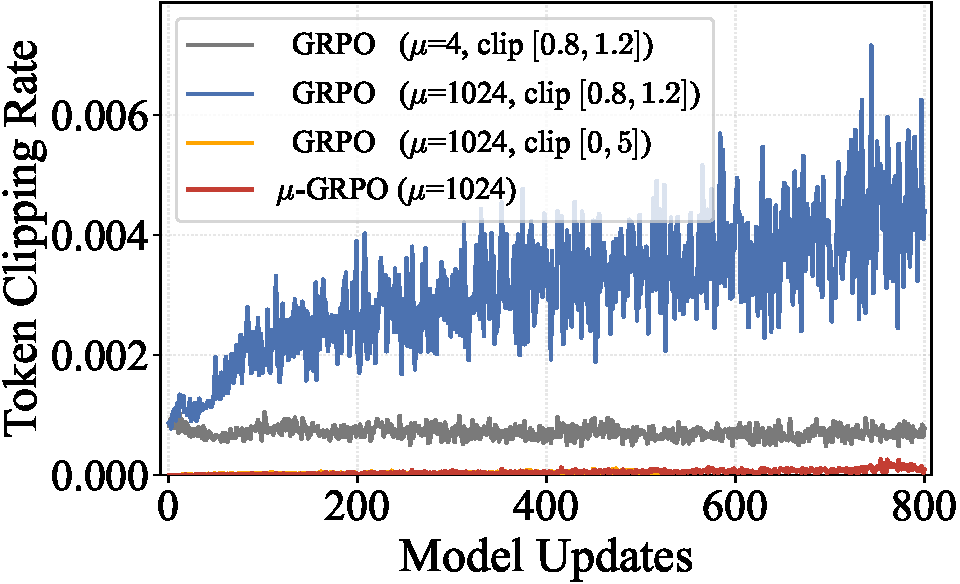
\includegraphics[width=0.48\textwidth]{figures/token_clipping.pdf}
%     \hfill
%     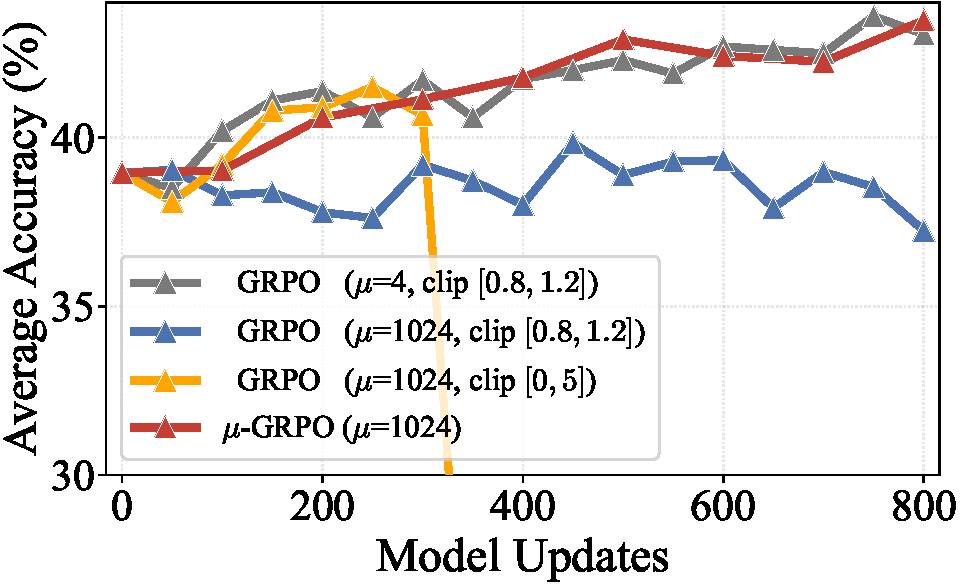
\includegraphics[width=0.48\textwidth]{figures/performance_comparison.pdf}
%     \caption{
%     \textbf{Training stability and performance of GRPO variants and \boldmath \ourmethod.}
%     (\textit{Left}) Token clipping ratio dynamics during training.
%      Large-$\mu$ GRPO with clipping exhibits a growing clipping rate, while \ourmethod\ keeps clipping near zero.
%     (\textit{Right}) Average accuracy over five math benchmarks. Relaxed clipping improves early learning but becomes unstable, whereas \(\mu\)-GRPO maintains stable training and achieves the best final accuracy. Experiments are conducted on Qwen-2.5-Math-7B.}
    
%     \label{fig:grpo_clipping_and_performance}
% \vspace{-1em}

% \end{figure*}

\begin{wrapfigure}{r}{0.65\textwidth}
\vspace{-1.0em}
\centering
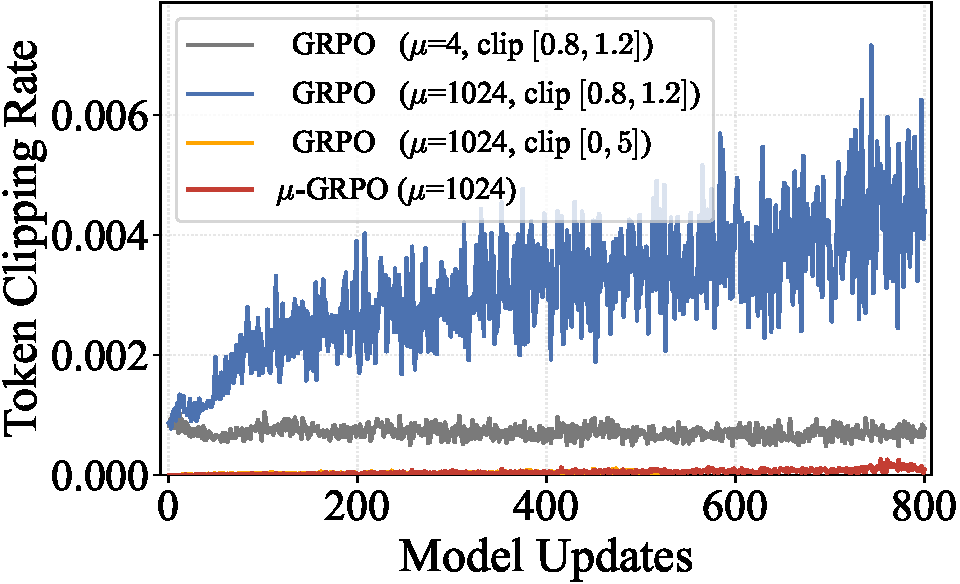
\includegraphics[width=0.32\textwidth]{figures/token_clipping.pdf}
\hfill
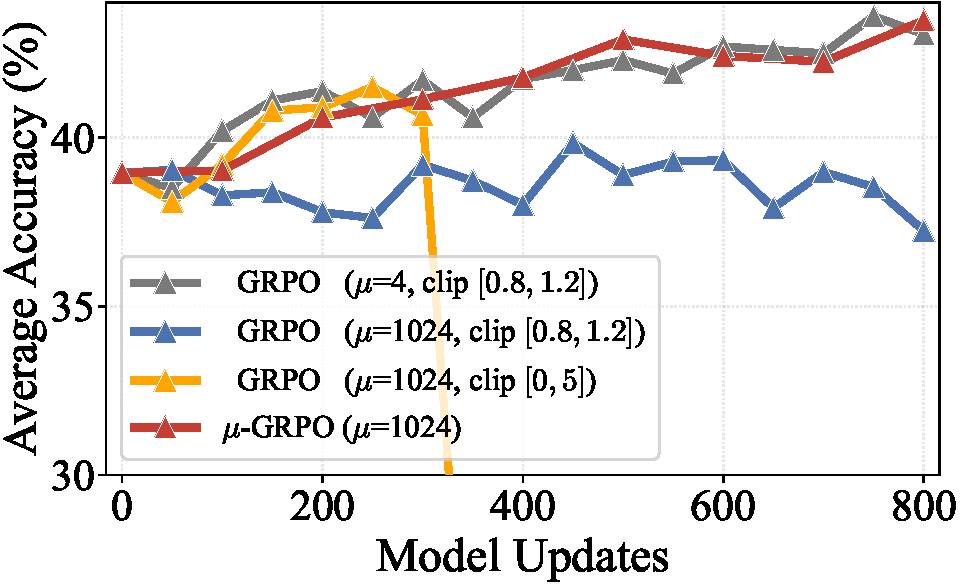
\includegraphics[width=0.32\textwidth]{figures/performance_comparison.pdf}
\vspace{-1.5em}
\caption{\textbf{Clipping creates a high-staleness dilemma.}
At $\mu=1024$, $[0.8,1.2]$ bound clips many more tokens and plateaus at lower accuracy ({\color{plotblue}blue}), while relaxed clipping recovers early gains but later collapses ({\color{plotyellow}yellow}).
Results are on Qwen2.5-Math-7B.}
\label{fig:grpo_clipping_and_performance}
\vspace{-1em}
\end{wrapfigure}